\chapter{Experiments}\label{ch:experiment}

\section{Simulated scenario}

To run experiments both in simulation and on real robots, this thesis implements a simulated scenario of a factory warehouse with one \gls{amr} and obstacles. The simulation is recorded and replayed for each experiment run to reduce the computation overhead of the simulation and to make the experiment repeatable. Furthermore, in order to compare the results from the simulation and the real robot, the simulation recording is used as input for both experiments under the same replay settings. 

\subsection{Environment}

% include a bird-view shot for the simulation with warehouse, robot, and human obstacles in the view.
The scenario simulates a modern-day factory warehouse, illustrated in (refer to the figure here). The simulated scenario is implemented in \gls{gazebo} with the help of a software package called "scenario execution", which the author implemented during his work at Intel Labs. The scenario consists of a factory warehouse environment and static obstacles, such as humans, boxes, shelves, and pallets, which are common obstacles in a factory warehouse. Since the object detection models are pre-trained with \gls{coco} data sets, which do not contain many of the static obstacles. The evaluation for the \gls{map} of the object detection task is restricted only to detecting human obstacles. To clarify, the object detection models still detect all of the classes that are defined in the \gls{coco} data sets. However, only the human class is taken into consideration when calculating the \gls{map} metric during the evaluation. Since the performance difference among different \gls{yolov5} models are negligible when the scene is too simple, this thesis includes ten human obstacles in the simulated scenario to increase the complexity of the object detection task. Moreover, some human obstacles are occluded by other obstacles in the scenario. Detecting occluded objects has been proven to be a challenging task in object detection. 

\begin{figure}
    \centering
    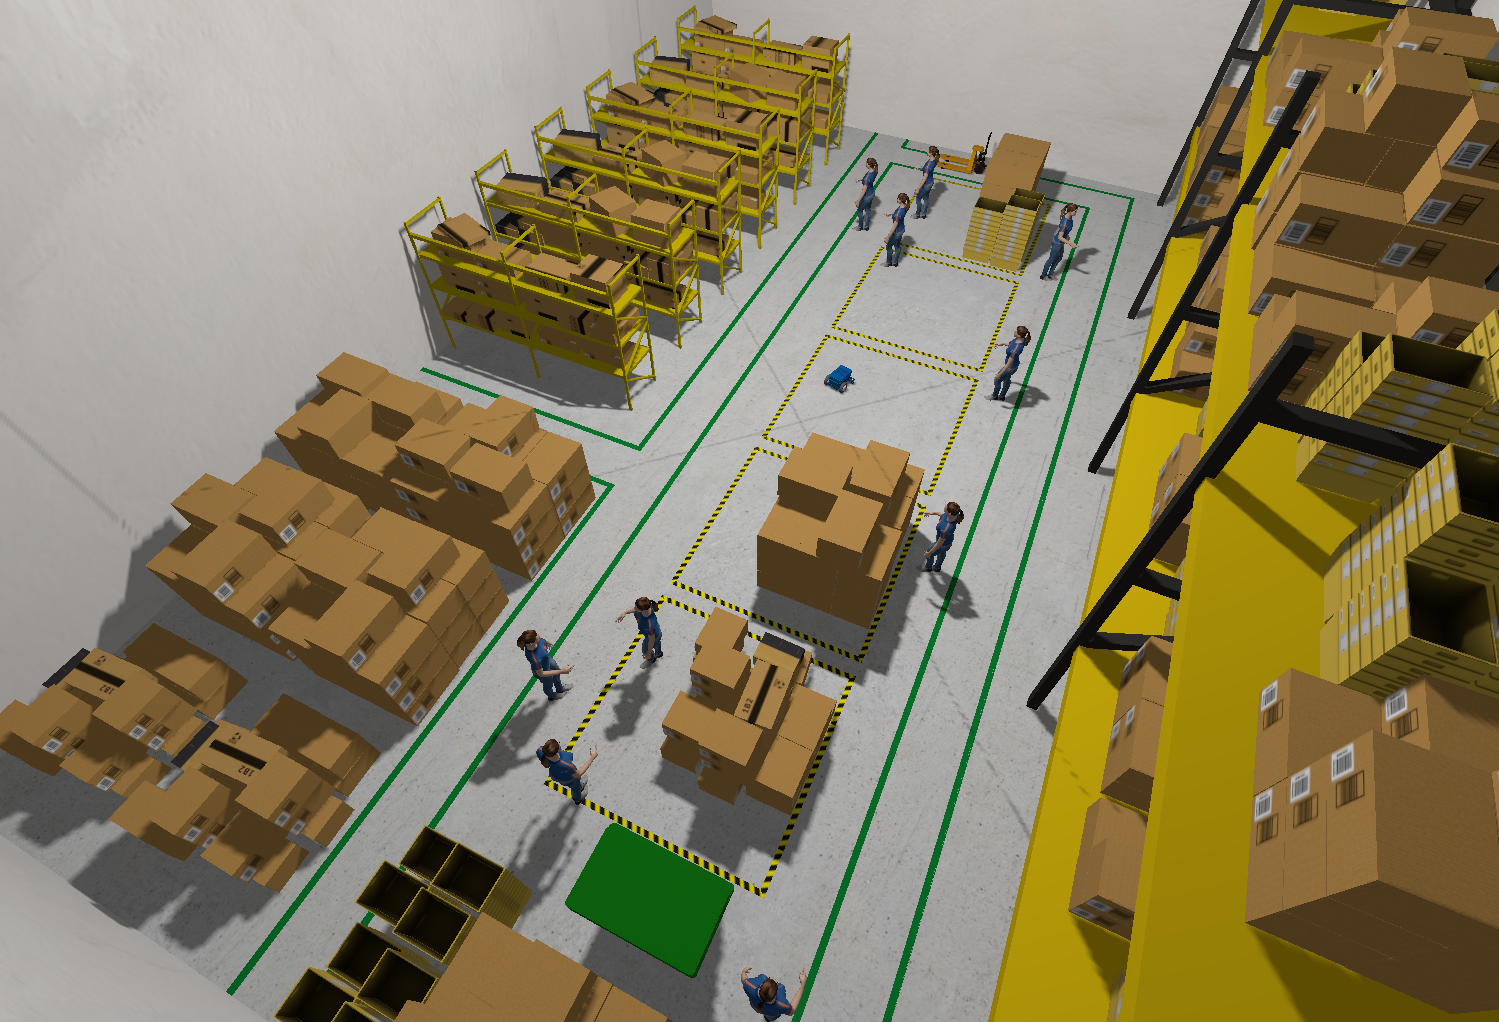
\includegraphics[width=\linewidth]{figures/sim/bird_view.png}
    \caption{Bird view of the simulated scenario}
    \label{fig:bird_view_scenario}
\end{figure}

\subsection{Robot}

The \gls{amr} is implemented as a dynamic obstacle in the scenario and it moves along a pre-defined path. The pre-defined path is made up of a series of waypoints in the simulation. Once the \gls{amr} reaches the current waypoint, the scenario execution will assign the next waypoint to the \gls{amr}. After all waypoints are successfully reached, the scenario execution shuts down the simulation. In the simulation, the \gls{amr} does not collide with other obstacles. The \gls{amr} is equipped with an RGB camera that is located on top of the robot and facing forward. The intrinsic parameters of the RGB camera sensor are listed in \cref{tab:camera_params}. During the simulation, the camera can observe all of the obstacles in the simulation with partial occlusion of some obstacles. In addition to the RGB image stream, the simulated camera sensor also outputs an image stream that contains the ground truth for the bounding boxes in the object detection task using the bounding box sensor from \gls{gazebo}. The ground truth data and the image stream are bridged from the \gls{gazebo} simulation topics to \gls{ros} topics so that the offloading pipeline can make use of them. In \cref{fig:robot_view_scenario}, it shows from the point of view of the \gls{amr}'s camera sensors. On the left, it shows the illustration of the bounding box ground truth data, while the image stream is shown on the right. The bounding box camera sensor and the RGB camera sensor are positioned the same and intend to simulate an actual point of view of a normal \gls{amr}.

\begin{table}[htp]
    \centering
    \begin{tabular}{lc}
    \toprule
    Parameter&                  Value\\
    \midrule
    Height&                     848 pixels\\
    Width&                      480 pixels\\
    FOV&                        1.047\\
    Frame rate&                 30 frames/sec\\
    Noise type&                 Gaussian\\
    Noise mean&                 0\\
    Noise standard deviation&   0.007\\
    \bottomrule
    \end{tabular}
    \caption{RGB camera intrinsic parameters}
    \label{tab:camera_params}
\end{table}

% describes how the robot is navigated, describes how the camera is mounted on the robot

\begin{figure}
    \centering
    \begin{subfigure}[h]{0.45\linewidth}
        \centering
        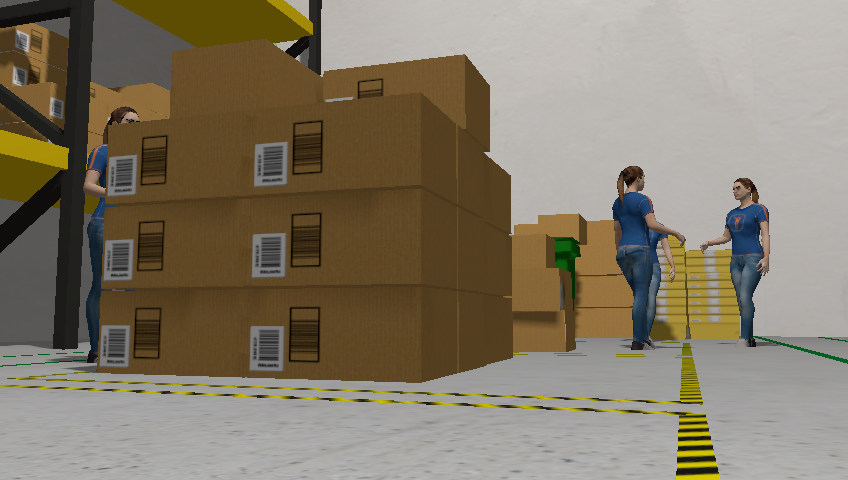
\includegraphics[width=\linewidth]{figures/sim/rgb_img.png}
        \caption{RGB image}
        \label{fig:robot_view_scenario:rgb_image}
    \end{subfigure}
    \begin{subfigure}[h]{0.45\linewidth}
        \centering
        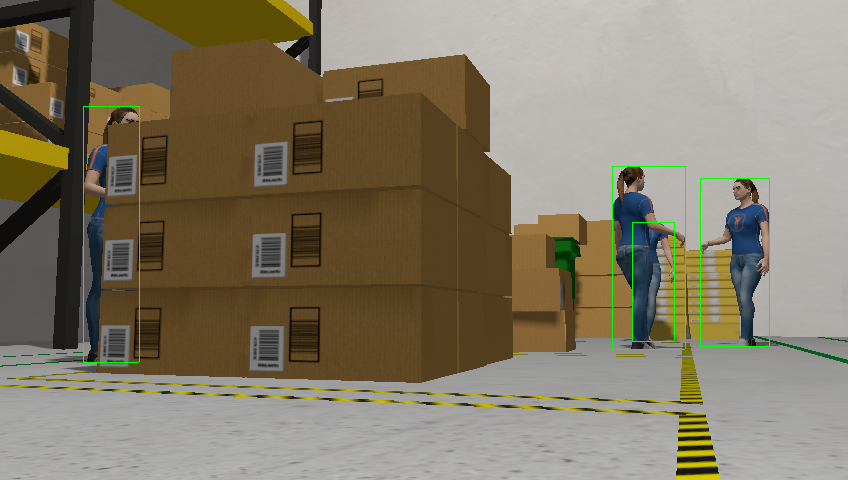
\includegraphics[width=\linewidth]{figures/sim/bbgt.png}
        \caption{Bounding box ground truth}
        \label{fig:robot_view_scenario:bbgt}
    \end{subfigure}
    \caption{Robot view of the simulated scenario}
    \label{fig:robot_view_scenario}
\end{figure}

It is worth pointing out that no dynamic obstacles are implemented in the simulated scenario. However, the \gls{amr} is dynamic and the camera sensors are mounted on top of it. Therefore, in the viewpoint of the \gls{amr}, the obstacles are constantly moving and thus could be treated as dynamic solely for the object detection task. Another reason for this is that the fresh out-of-box bounding box sensor from \gls{gazebo} is inaccurate for dynamic obstacles like humans because dynamic human actors are implemented as the actors in \gls{gazebo} and the animation of the actors is realized by the deformation of the meshes of the actor model. Unfortunately, the bounding box sensor can only provide the bounding boxes of the undeformed actor. Therefore, the bounding boxes available are not accurate to serve as the ground truth for the object detection task. Till the finish of the thesis, the problem is not resolved with the current version of \gls{gazebo} this thesis uses. However, static human obstacles and dynamic \gls{amr} still constitute an adequate simulated scenario for the research questions this thesis is trying to address. 

\subsection{Record and Replay}

% describes how the ROS bag is recorded and how is it replayed during the experiments and explain why this is needed. 
The simulation takes up a great amount of the resources of computers. To reduce the overhead of running the simulation alongside the experiments, this thesis records the simulation to a \gls{ros} bag and replays it during the experiment runs. This reduces the \gls{cpu} and memory usage of the host machine during the experiment and improves the performance of the rest of the offloading pipeline. As mentioned in (TODO: add a reference here), \gls{ros} provides the functionality to record the topics and allows the users to replay them later while preserving the same publishing rate and order of the messages. More importantly, this thesis conduct experiment on a real robotic system with limited resources. Such a system is not capable of running real-time simulations while maintaining the rest of the offloading pipeline. In real-world applications, \glspl{amr} only needs to maintain the driver of the camera and minimal software to be able to get the same image input. In \cref{tab:ros_bag_comparison}, this thesis presents an experiment comparing the \gls{cpu} usage of replaying a \gls{ros} bag and running the library for the Intel RealSense camera. The results show that the two processes have comparable \gls{cpu} usage on a robotic system. Furthermore, \gls{gazebo} slows down the simulation time compared to real-time when the system is strained. Therefore, to ensure a real-time simulation, specifying a replay rate of the \gls{ros} bag can guarantee the simulation time factor is within a reasonable range. 

\begin{table}[htp]
    \centering
    \begin{tabular}{lc}
    \toprule
    Process&                    CPU usage\\
    \midrule
    \gls{ros} bag replay&       14.12\%\\
    RealSense camera library&   11.28\%\\
    \bottomrule
    \end{tabular}
    \caption{Comparison of CPU usage on robotic system}
    \label{tab:ros_bag_comparison}
\end{table}

All topics during the simulation are recorded in the \gls{ros} bag, including the RGB images, the bounding box ground truth, the camera information, etc. The image stream consists of 1748 frames and the \gls{ros} bag is replayed at around 25 frames per second during the experiment. Topics for RGB image stream and the bounding box ground truth are replayed with best effort reliability setting to ensure the RGB images are replayed the same way it is recorded. Since the \gls{ros} topics are recorded at a different time than the experiment, the time stamps of the RGB image messages and the ground truth messages have to be overwritten by the receiving time of the offloading module.

% ---------------------------------------------------------------
\section{Experimental Setup}\label{sec:experiment:experiment_setup}
% ---------------------------------------------------------------

\subsection{Simulation experiment setup}

The host machine is equipped with an Intel(R) Core(TM) i9-7900X \gls{cpu} and a Nvidia GeForce GTX 1060 6GB \gls{gpu}. The \gls{cpu} has a total of 20 cores. In order to simulate the \gls{amr}'s and the edge computer in realistic conditions, this thesis limits the computation resources of the \gls{docker} containers. The robot container is constrained to using only eight cores of the host machine, while the edge container is given ten cores. In addition, the edge computer has the access to the \gls{gpu} of the host machine and calculates the image inference on the \gls{gpu}. Moreover, the robot container is also constrained to using only 4 GB of memory, while the memory of the edge container is not constrained and the host machine has access to 32 GB of memory, including the 4 GB memory assigned to the robot container.

The limitations of CPU and memory usage are realized by tools provided by \gls{docker} itself. According to the \gls{docker} documentation, the runtime memory limitation is realized by Memory Resource Controller provided by the \gls{linux} kernel. Furthermore, the \gls{docker} container can enforce hard memory limitation and soft memory limitation at runtime. The former does not allow the container to use any amount more than specified, while the latter only kicks in when certain conditions are met. In this thesis, we use the hard memory limitation on the robot container to simulate the hardware constraints. For CPU usage, the limitation is realized by the CFS scheduler, which is the \gls{linux} kernel CPU scheduler for normal \gls{linux} processes. This indicates that the limitation on CPU usage is achieved by limiting the accessible CPU cycles of the \gls{docker} container. The GPU of the host machine is exposed to the \gls{docker} containers using the Nvidia Container Toolkits.

In addition to resource limitation simulation, the network is also simulated to achieve realistic conditions for the robot and edge containers. The containers use the default \gls{docker} bridge network. Since the simulated scenario \gls{ros} bag is replayed in the robot container and the output data are also recorded in the robot container, the data flow between the robot container and the edge container only consists of offloaded images and detection processed by the edge container. To allow the data flow of 30 frames per second of images with resolution of 848 x 640 pixels, which is around 40 MB per second, the packet limit of in and out policies of the \gls{netem} is set to 20000. The in and out delays are set to 50 ms for both policies. To investigate the influence of the network bandwidth, the experiments are carried out under two bandwidth conditions: with 160 Mbit/s bandwidth constraint and no bandwidth constraints at all. The former aims to represent a limited network bandwidth that is unable to handle the data flow that is needed for a full offloaded execution, while the latter one represents a unlimited network bandwidth. 

For \gls{qos} settings, the offloading module uses "best effort" reliable policy to prevent the the publisher from being blocked by the bag network connection caused by the bandwidth constraints. As mentioned in (TODO: add a reference here), only \gls{fast_dds} allows a true asynchronous publishing mode. Therefore, Fast-DDS is used for \gls{ros} middle ware and the publishing mode is set to asynchronous for the experiments. The offloading module uses the "keep last" queuing settings and the queue size is set to 5. Furthermore, the \gls{ros} bag replay of the simulated scenario and the state monitors also use "best effort" reliable policy settings to simulate a camera sensor. 

\subsection{Robot experiment setup}

Unlike the simulation experiments, described in (TODO: add a reference here), the real-robot experiment uses two separate computers for the \gls{amr}'s onboard system and the edge computer. For the robot, the onboard system uses a \gls{nuc} equipped with an Intel(R) Core(TM) i3-8109U \gls{cpu}, which is commonly used for \glspl{amr}.  For the edge, a \gls{linux} desktop computer equipped with an Intel(R) Core(TM) i3-8109U \gls{cpu} and a Nvidia GeForce GTX 1060 6GB \gls{gpu} is used. On both computers, the offloading module and the perception modules have full access to the available resources. The distribution of the modules between the two computers is illustrated in (TODO: add a reference here). The \gls{ros} bag replay of the simulated scenario is carried out on the robot. The output data of the metrics are also recorded on the robot. The edge computer is solely responsible for the inference of the offloaded images and monitoring the edge system states and sending them to the robot. The image inference is computed by the \gls{gpu} on the edge computer with help of \gls{pytorch} library, while the image inference on the robot is computed by its onboard \gls{cpu}. As mentioned in (TODO: add a reference here), the system states of the robot and the edge are measured with the "system status" package.

% TODO: add a photo of nuc is this figure
% \begin{figure}
%     \centering
%     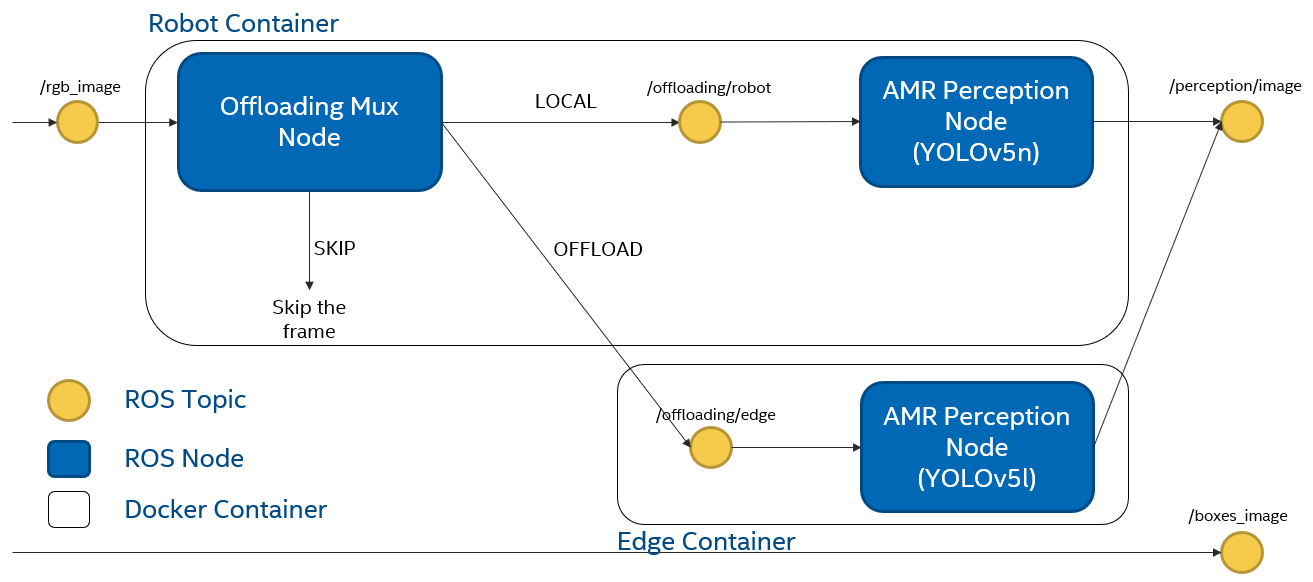
\includegraphics[width=\linewidth]{figures/setup/general_setup.png}  % TODO: change here
%     \caption{Setup for real-robot experiment (TODO: adapt this fig)}  % TODO: change here
%     \label{fig:real_robot_experiment_setup}  % TODO: change here
% \end{figure}

Two network interfaces are used to conduct the real-robot experiments. First, the experiment uses an Ethernet connection between the two computers. Similar to the simulation experiments, two network conditions are tested under the Ethernet connection. First, an Ethernet network interface without bandwidth constraints is used to simulate a perfect network connection between the robot and the edge. Then, the Ethernet network interface is constrained to 160 Mbits/s bandwidth to simulate a bag network connection. Finally, a \gls{wifi} network interface is used the carry out the experiment. The \gls{wifi} network has unstable network bandwidth from time to time and therefore affects the experiment results drastically. This is to investigate different offloading strategies under dynamic network condition changes. When conducting the experiment with one network interface, the other one is shutdown to avoid the offloading pipeline uses both network interfaces simultaneously. 

Similar to simulation experiment, \gls{fast_dds} is used as middle ware for \gls{ros}.The \gls{qos} reliability policy for offloading is set to "best effort" and the publishing mode of \gls{fast_dds} is set to asynchronous to avoid the publisher blocked by the network. Moreover, the queuing settings use "keep last" policy and the queue size is set to five messages. Under various \gls{qos} settings, this setup achieves the best performance of the object detection task. However, other \gls{qos} settings are also investigated during the experiments. In (TODO: add a reference here), the results of the experiment with "reliable" reliability policy are presented. 


\section{Evaluation Framework}

\subsection{Metrics}
% This section lists all the evaluation metrics used and how they are recorded and what tools are used in order to record them. 

% TODO: rewrite this section with more specifications on how the metrics are measured. Maybe list all metrics in itemized order. 

The evaluation metrics used by this thesis fall into two categories. The second category focuses mainly on the resources of the \gls{amr}. This includes the CPU percentage, the power consumption, and the network throughput. These metrics represent the onboard resources for computation, energy, and network used by the \gls{amr}. For these metrics, this thesis also includes the results when the offloading pipeline is idling as a baseline to eliminate the influence of processes other than the perception modules on the metrics. More specifically, in the baseline, the offloading module and the perception modules are still launched and the ROS bag is also being replayed. However, the offloading module is not sending any messages to the onboard perception module or the edge perception module, i.e., there are no object detection tasks being performed at all. 

The second category describes the performance of the object detection task, including the execution latency, the overall processed frame rate, and the \gls{map}. The two components of the execution latency, i.e., the network delay and the inference time, are evaluated separately for offloading and local computation. In addition, to evaluate how the offloading pipeline is performing over the entire simulation, the overall processed frame rate, i.e., what percentage of all the frames are processed by perception modules. The \gls{map} only consider the person class in the obstacles. The detection from the perception modules is compared with the bounding box ground truth from the simulation. The evaluation algorithm is provided by the package "torchauto" as a part of the code base from \gls{amsrl}. 

For the comparison between the detection and the ground truth, the time stamps of the messages are crucial to the final result. This raises the question: what should be considered as simultaneity for the detection and the ground truth in task offloading? This thesis presents two evaluation methods of the \gls{map} metric in order to gain some insights into this question. 

\subsection{Evaluation methods}

\begin{figure}[htp]
    \centering
    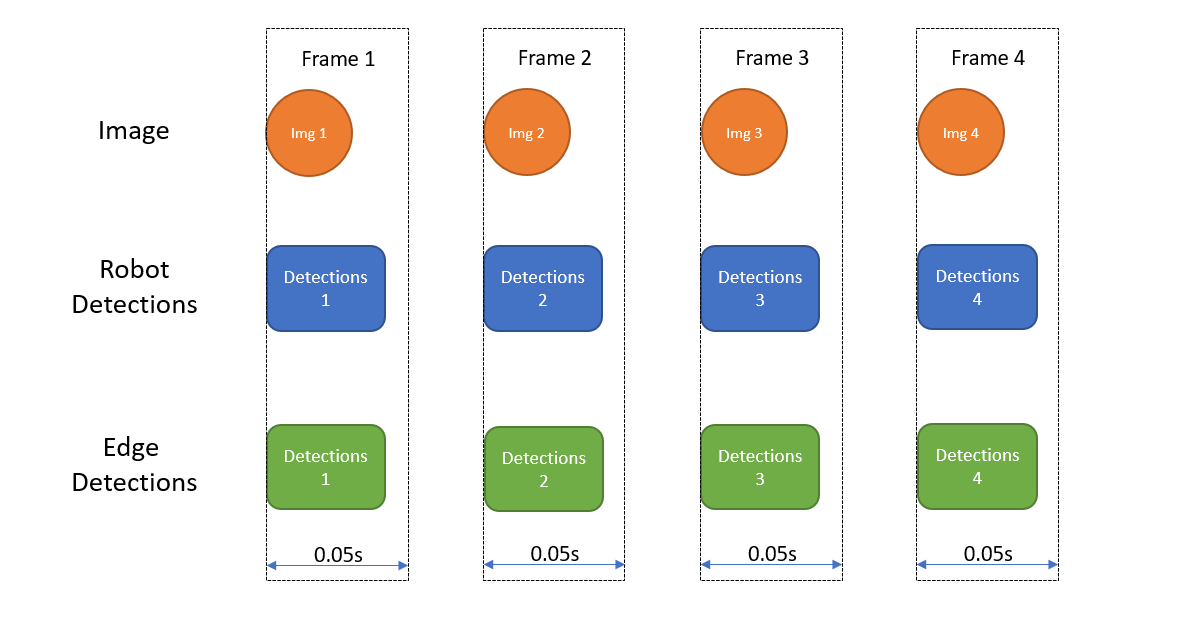
\includegraphics[width=\linewidth]{figures/setup/sync_eval.png}
    \caption{Synchronous evaluation}
    \label{fig:sync_eval}
\end{figure}

In the synchronous evaluation, the detection is evaluated by being compared with the ground truth of the same time stamp. As illustrated in \cref{fig:sync_eval}, the image is either processed by the robot perception module or the edge perception module. The processed result and the ground truth are recorded by the ROS bag. After the experiment runs, the recorded result and the ground truth with the nearest time stamps are grouped as one data frame by the message filter. The message filter groups the messages from different ROS topics. The proximate messages within a time threshold can be considered as the same data frame. The threshold is currently set to 0.05 seconds. The \gls{map} is calculated within the same data frame. For the entire experiment run, the mean and the standard deviation are calculated for all the data frames. This means the data frame is discarded if no detection or ground truth is present for the specific time stamp, i.e., the \gls{map} will not be affected if the robot onboard system or the edge computer is not capable of processing the image. The capability of processing the image is however reflected in the metric of the overall processed frame percentage. 

The synchronous evaluation method does not take the execution latency into consideration, because the detection is compared against the ground truth with the same time stamp as the original image. Therefore, the final result interpolates the \glspl{map} of the edge computer and the robot onboard system. However, this also does not represent the offloading scenario accurately. In real-world applications, the \glspl{amr} move continuously. The current situation of the \gls{amr} could be very different than the moment the image is taken by the camera if the processing takes too long and the detection is outdated. Therefore, the execution latency plays an important role in the accuracy of how well the \glspl{amr} perceives the environment. 

With the aforementioned considerations, this thesis investigates an asynchronous evaluation method that takes the execution latency into consideration, which is the evaluation method for \gls{map} metric that the thesis adopts. As illustrated in \cref{fig:async_eval}, the detection is compared against the images with the time stamps when the \glspl{amr} actually receive the processed result. This is achieved by changing the time stamps of the detection messages to the receiving time of the \glspl{amr}. Depending on how much the images have changed, the quality of the detection deteriorates with the execution latency, which is usually the case in real-world applications.

\begin{figure}[htp]
    \centering
    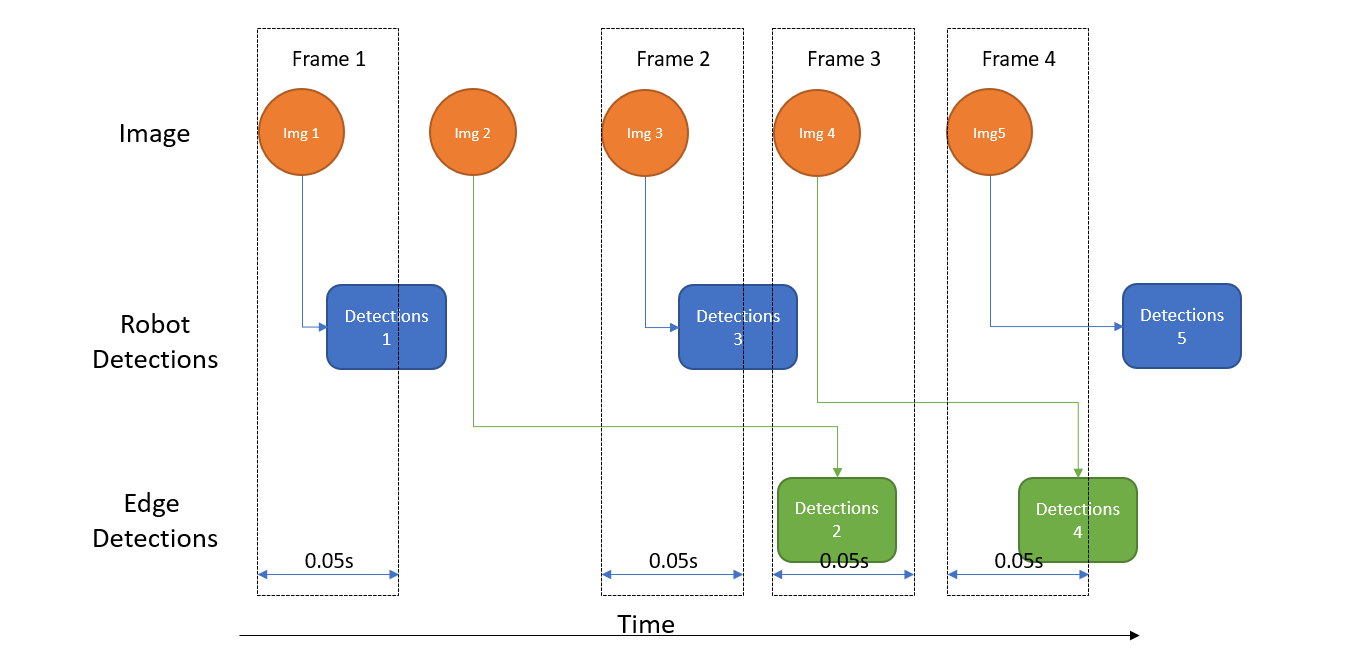
\includegraphics[width=\linewidth]{figures/setup/async_eval.png}
    \caption{Asynchronous evaluation}
    \label{fig:async_eval}
\end{figure}

% -----------------------------------------------
\section{Analysis}\label{sec:experiment:analysis}
% -----------------------------------------------

\subsection{Simulation experiment}

\subsection{Robot experiment}

When the network condition is not constrained, the "edge only" strategy shows the best results in the object detection task, as shown in \cref{fig:real_robot_experiment:eth_map}. This is mainly caused by two reasons. On one hand, the edge computer is using the more complex network, i.e., \gls{yolov5}l, which provides a more precision detection. On the other hand, even though the \gls{rtt} of the edge perception is still higher than the robot perception, the difference is still relatively low, as shown in \cref{fig:real_robot_experiment:eth_rtt}. Therefore, the inaccuracy caused by the execution delay is negligible. Moreover, the "edge only" strategy also processed the most frames in the experiments. This also makes the "edge only" strategy the safest among different strategies. With more detection frames, the \gls{amr} is able to adapt its behavior to the detection more quickly. The "edge only" strategy also uses the least \gls{cpu} and energy of the onboard system, since the images are exclusively calculated on the edge computer. This is beneficial to \gls{amr}'s onboard system and battery life. This also allows the \glspl{amr} to free up more resources for other tasks, e.g., \gls{slam}, navigation, and path planning. However, the "edge only" strategy also uses the most network bandwidth. For image feed with 30 \gls{fps} at a resolution of 848x640 pixels, around (TODO: add a number here) MB/s bandwidth is used for offloading. Such bandwidth will be a huge amount for wireless connection. For comparison, IEEE IEEE 802.11ac (\gls{wifi} 5G) can support only up to (TODO: add a number here) bandwidth. If the number of the \glspl{amr} scales, the network cannot provide such bandwidth. Therefore, "edge only" strategy is not suitable for industrial usage. 

% Figure for eth mAP
\begin{figure}
    \centering
    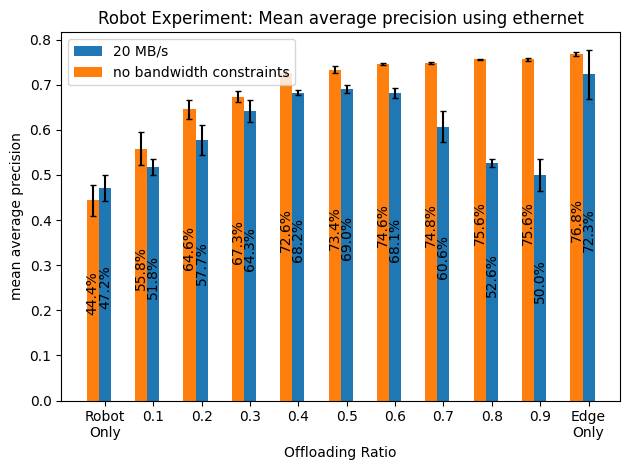
\includegraphics[width=\linewidth]{figures/experiment/real_robot/eth/map.png}
    \caption{Real-robot experiment: \gls{map} with Ethernet}
    \label{fig:real_robot_experiment:eth_map}
\end{figure}

On the other hand, the "robot only" strategy delivers the worst results in the object detection task. This is mainly because the onboard resources are not enough for the \gls{amr} to process all the images. The robot perception module is strained when more images are calculated locally on the \gls{amr}'s onboard system. As shown in \cref{fig:real_robot_experiment:eth_rtt}, the robot perception has the highest \gls{rtt} with "robot only" strategy. The \gls{rtt} of robot perception is broken down to different components in \cref{fig:real_robot_experiment:eth_execution_time_320}. The inference time of the robot perception stays the same. However, the network delay is increased. This indicates that the robot perception module has too many images waiting for processing and the images start to queue, causing the network latency of robot perception to increase. As shown in \cref{fig:real_robot_experiment:eth_execution_time_320}, the network latency of robot perception stabilizes around 0.6 offloading ratio. This infers that the \gls{amr}'s onboard system, i.e., the \gls{nuc}, is only able to process less than 40 percent of the offloaded images, i.e., around 12 \gls{fps}. This corresponds to the 99.9 ms \gls{rtt} of the robot perception at offloading ratio 0.6, as shown in \cref{fig:real_robot_experiment:eth_rtt}. Naturally, the "robot only" strategy also uses the most \gls{cpu} and energy, since it computes the all images onboard, as shown in \cref{fig:real_robot_experiment:eth_cpu_percentage} and \cref{fig:real_robot_experiment:eth_cpu_energy_consumption}. Moreover, the "robot only" strategy uses the least network bandwidth. It still uses 0.4 MB/s network bandwidth because the states monitors need to send system state data from the edge computer to the \gls{amr}'s onboard system.

As illustrated in \cref{fig:real_robot_experiment:eth_map}, the \gls{map} of the object detection task saturates between offloading ratios 0.5 and 0.8. This indicates that both the robot perception and the edge perception are working under their optimal workload. The task performance reaches a stationary point. After the stationary point, the edge perception becomes more prominent for the performance. Therefore, the performance continues to improve due to the more accurate object detection of the more complex model on the edge. 

The decision-making strategy also delivers decent results for the object detection task under good network condition. As shown in \cref{fig:real_robot_experiment:eth_processed_frame_percentage_320}, the decision-making strategy offloads most images to the edge computer and only computes (TODO: add a number here) on the \gls{amr}'s onboard system. This decision can be justified by the low \gls{rtt} of the edge computer. (TODO: add analysis after getting the results). It it worth noticing that decision-making strategy calculates a small portion of the images locally on the onboard system, since the \gls{rtt} of edge perception can increase temporarily due to dynamic changes in the network. However, because the network condition is good, most of the images are offloaded to the edge computer. 

% Figure for eth RTT
\begin{figure}
    \centering
    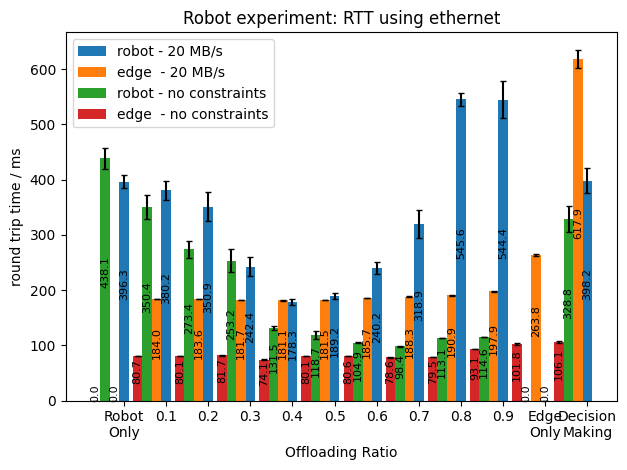
\includegraphics[width=\linewidth]{figures/experiment/real_robot/eth/RTT.png}
    \caption{Real-robot experiment: \gls{rtt} with Ethernet}
    \label{fig:real_robot_experiment:eth_rtt}
\end{figure}

When the network condition is constrained, the "edge only" strategy does not provide the best \gls{map} among all strategies. Since the network is not capable of transmitting the amount of data the strategy needs, the messages starts to queue and the "best effort" reliable policy allows the middleware to drop many messages. This can be visualized in \cref{fig:real_robot_experiment:eth_execution_time_160} and \cref{fig:real_robot_experiment:eth_processed_frame_percentage_160}. The processed frame percentage starts to drop drastically after the offloading ratio exceeds 0.5 and the network latency of the edge perception increases. This also corresponds to the network bandwidth in \cref{fig:real_robot_experiment:eth_bandwidth}. The network bandwidth is at its capacity after the offloading ratio exceed 0.5. Furthermore, with the offloaded images hogging the network bandwidth, it is unlikely for the \glspl{amr} to transmit other data over the network, which can be essential for the safety of the \glspl{amr}. This makes "edge only" strategy the worst strategy under constrained network condition. 

On the other hand, the "robot only" strategy delivers similar results under the two network conditions. Since the "robot only" strategy compute the object detection locally on the onboard system, the performance should be independent from the network conditions. However, it is worth noticing that the there is a slight performance drop for all strategies up to offloading ratio 0.5 due to a slight increase of the network latency on the robot perception. It is suspected that the \gls{netem} layer affects the \gls{ros} middleware and thus causes a increased latency in transmitting the data between the offloading module and the robot perception module. 

The best performance of \gls{map} occurs around offloading ratio of 0.5. At this offloading ratio, the network bandwidth has not exceeded its limits and the robot perception is able to process the given workload. Therefore, the \glspl{rtt} of both perception modules are low and the \gls{amr} is able to get the detection in time. Moreover, offloading at this ratio also allows the \gls{amr} to use less onboard resource, as shown in \cref{fig:real_robot_experiment:eth_cpu_percentage} and \cref{fig:real_robot_experiment:eth_cpu_energy_consumption}. Therefore, under constrained network condition, offloading a portion of the images is the best strategy. However, the offloading ratio is dependent on the available network bandwidth and the computation capabilities of the \gls{amr}'s onboard system.

% Under constrained network condition, the decision-making strategy also managed to deliver decent results. The increased \gls{rtt} time forces the \gls{amr} to compute most of the images locally. However, the decision-making strategy still offloads a portion of the images to the onboard system, because the onboard system is not able to process all images and \gls{rtt} of the robot perception will increase drastically if the images start to queue. These results show that the decision-making strategy is able adapt to the dynamic changes of the network by simply using the \gls{rtt} as a criterion. Furthermore, the \gls{amr} uses more \gls{cpu} and energy with the decision-making strategy under constrained network condition compared to unconstrained network condition, since the \glspl{amr} have to do more computation on the board system and thus consume more onboard resources, as shown in \cref{fig:real_robot_experiment:eth_cpu_energy_consumption} and \cref{fig:real_robot_experiment:eth_cpu_percentage}.

% Figure for eth execution time 160M
\begin{figure}
    \centering
    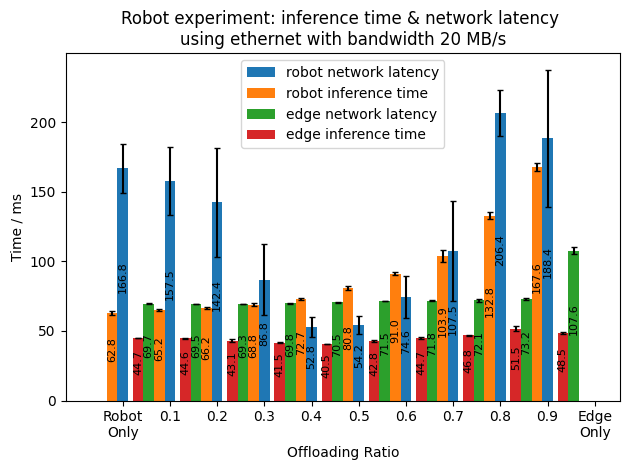
\includegraphics[width=\linewidth]{figures/experiment/real_robot/eth/execution_time_160.png}
    \caption{Real-robot experiment: execution times with Ethernet with 160 Mbits/s bandwidth}
    \label{fig:real_robot_experiment:eth_execution_time_160}
\end{figure}

% Figure for eth execution time 320M
\begin{figure}
    \centering
    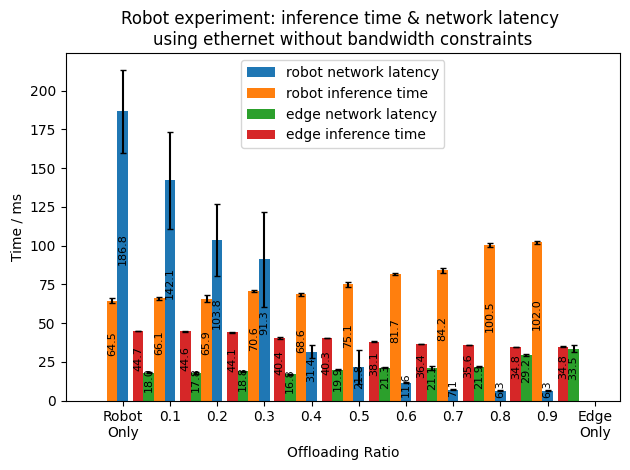
\includegraphics[width=\linewidth]{figures/experiment/real_robot/eth/execution_time_320.png}
    \caption{Real-robot experiment: execution times with Ethernet with 320 Mbits/s bandwidth}
    \label{fig:real_robot_experiment:eth_execution_time_320}
\end{figure}

% Figure for eth overall processed image percentage
\begin{figure}
    \centering
    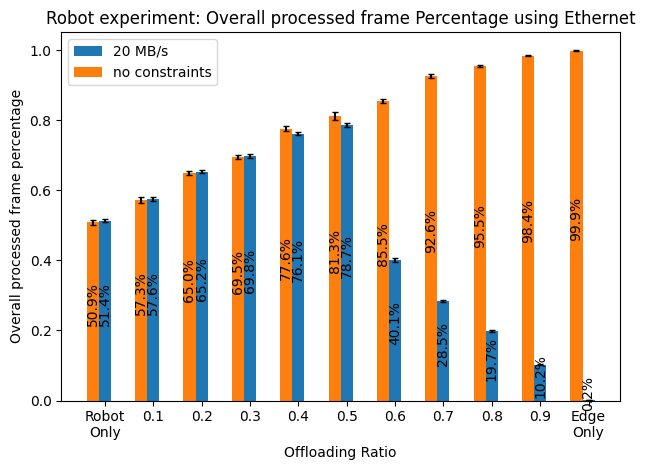
\includegraphics[width=\linewidth]{figures/experiment/real_robot/eth/overall_processed_frame_percentage.png}
    \caption{Real-robot experiment: overall processed frame percentage with Ethernet}
    \label{fig:real_robot_experiment:eth_overall_processed_frame_percentage}
\end{figure}

% Figure for eth processed image percentage 160M
\begin{figure}
    \centering
    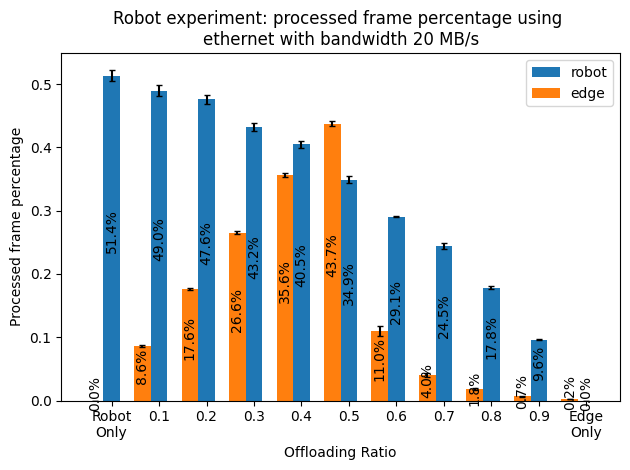
\includegraphics[width=\linewidth]{figures/experiment/real_robot/eth/frame_percentage_160.png}
    \caption{Real-robot experiment: processed percentage with Ethernet with 160 Mbits/s bandwidth}
    \label{fig:real_robot_experiment:eth_processed_frame_percentage_160}
\end{figure}

% Figure for eth processed image percentage 320M
\begin{figure}
    \centering
    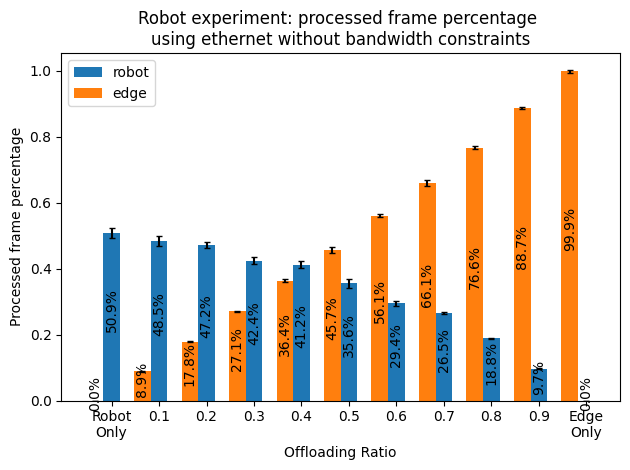
\includegraphics[width=\linewidth]{figures/experiment/real_robot/eth/frame_percentage_320.png}
    \caption{Real-robot experiment: processed percentage with Ethernet with 320 Mbits/s bandwidth}
    \label{fig:real_robot_experiment:eth_processed_frame_percentage_320}
\end{figure}

% Figure for CPU percentage
\begin{figure}
    \centering
    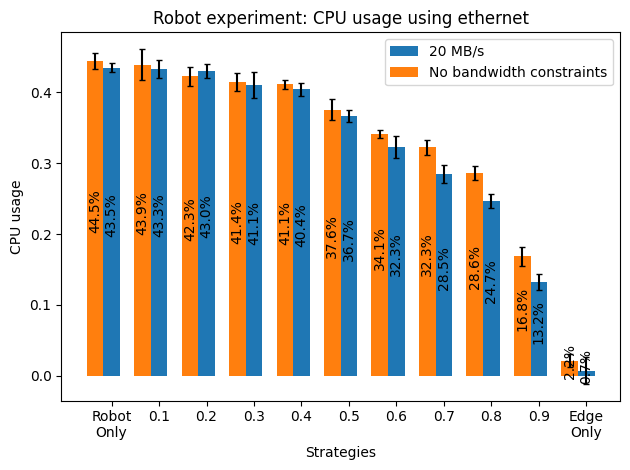
\includegraphics[width=\linewidth]{figures/experiment/real_robot/eth/cpu_percentage.png}
    \caption{Real-robot experiment: CPU usage using Ethernet}
    \label{fig:real_robot_experiment:eth_cpu_percentage}
\end{figure}

% Figure for CPU energy consumption
\begin{figure}
    \centering
    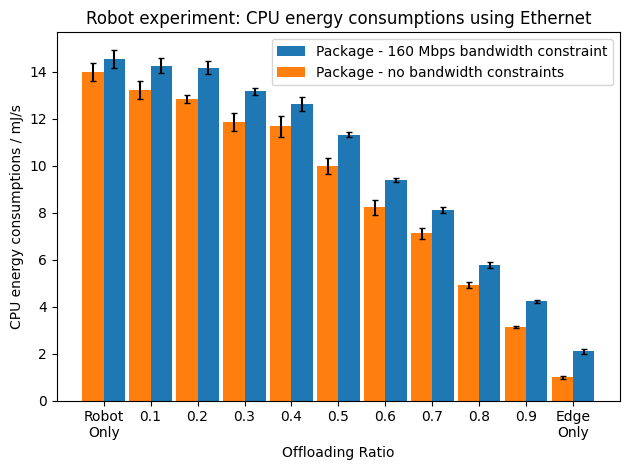
\includegraphics[width=\linewidth]{figures/experiment/real_robot/eth/cpu_energy_consumption.png}
    \caption{Real-robot experiment: CPU energy consumption using Ethernet}
    \label{fig:real_robot_experiment:eth_cpu_energy_consumption}
\end{figure}

% Figure for network bandwidth
\begin{figure}
    \centering
    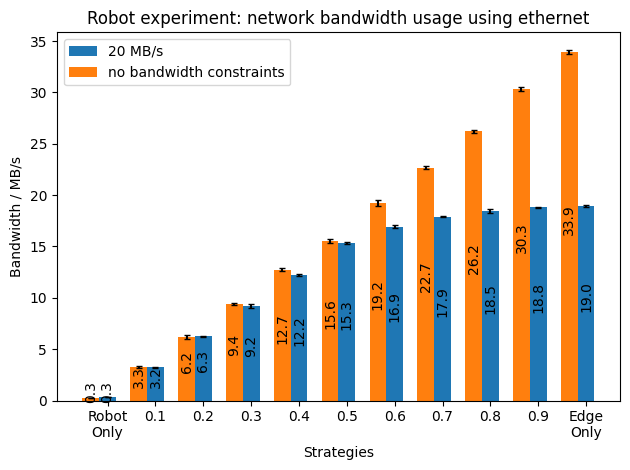
\includegraphics[width=\linewidth]{figures/experiment/real_robot/eth/bandwidth.png}
    \caption{Real-robot experiment: network bandwidth usage using Ethernet}
    \label{fig:real_robot_experiment:eth_bandwidth}
\end{figure}
